%! TEX root = ./fuss_catalan_area.tex
\documentclass[12pt]{article}

%--------Packages-------------
\usepackage[noquiver]{kyrem1sty}
%----------------------------


%--------Bibliography---------
\usepackage[backend=biber,style=alphabetic,doi=false,isbn=false,url=false,eprint=false]{biblatex}
\addbibresource{/home/kyrem1/Mathematics/bibs/comborefs.bib}
%----------------------------


%--------Hyper Setup-------
\hypersetup{%
  colorlinks=true,%
  linkcolor=blue,%
  citecolor=blue,%
  filecolor=blue,%
  menucolor=blue,%
  urlcolor=blue,%
  pdfnewwindow=true,%
  pdfstartview=FitBH
}   
%----------------------------


%--------Other Setup-------
\usepackage{tikz}

%\usetikzlibrary{arrows.meta,decorations.pathreplacing,positioning}
\usetikzlibrary{arrows.meta,calc,decorations.pathreplacing,positioning,decorations.markings}

\usepackage{ytableau} % For young diagrams
%\usepackage{todonotes}
%\newcommand{\Jenn}[1]{\todo[size=\tiny]{#1
%      \\ \hfill --- Jenn}}
\usepackage{caption}
% Adjust caption spacing and font
%\captionsetup{
%  font=small, % Adjust the font size
%  labelfont=bf,
%  format=plain, % Use plain format to avoid any unwanted effects
%  justification=raggedright, % Ensure the caption is justified, which can help with spacing
%  singlelinecheck=false, % Applies justification setting even when the caption is a single line
%}
%----------------------------


%--------Subfiles Setup-------
\usepackage{subfiles}
%----------------------------


%--------Page Setup-----------
%\usepackage{geometry}\geometry{margin=1in}
\pagestyle{empty}%

\setlength{\hoffset}{-1.54cm}
\setlength{\voffset}{-1.54cm}

\setlength{\topmargin}{0pt}
\setlength{\headsep}{0pt}
\setlength{\headheight}{0pt}

\setlength{\oddsidemargin}{0pt}

\setlength{\textwidth}{195mm}
\setlength{\textheight}{250mm}
%----------------------------


%--------Metadata------------
\title{The Total Area Statistic for Fuss-Catalan Paths}
\author{James Harbour}
%----------------------------


%--------Content-------------
\begin{document}
\maketitle
\tableofcontents


\section{Preliminaries}
\begin{tikzpicture}[scale=1,dot/.style={circle,fill,inner sep=1pt}]

    % Draw grid of dots
    \foreach \x in {0,...,12}
        \foreach \y in {0,...,6}
            \node[dot] at (\x,\y) {};

    % Draw axes
    \draw[thick,->] (-1,0) -- (13,0) node[anchor=north west] {$x$};
    \draw[thick,->] (0,-1) -- (0,7) node[anchor=south east] {$y$};
    
    % Draw the line x = μy (for some μ)
    \draw[domain=0:6,samples=100,variable=\y,ultra thick] plot ({\y*2},\y) node[anchor=south west] {$x=\mu y$};
    
    % Draw the path P with labels for S0, S1, and Sv
    \draw[thick] (0,0) -- (2,0) -- (2,1) -- (4,1) -- (4,2) -- (6,2) -- (6,3) -- (7,3) -- (7,4) -- (8,4) -- (8,5) -- (9,5);
    \node[dot,label=below:$S_0$] at (2,0) {};
    \node[dot,label=below:$S_1$] at (4,1) {};
    \node[dot,label=below:$S_2$] at (6,2) {};
    \node[dot,label={[xshift=2pt]above:$S_v$}] at (9,5) {};

    % Draw braces and labels for P0, P1, P2
    \draw[decorate,decoration={brace,mirror,raise=5pt}] (0,0) -- node[below=10pt] {$P_0$} (2,0);
    \draw[decorate,decoration={brace,mirror,raise=5pt}] (2,1) -- node[below=10pt] {$P_1$} (4,1);
    \draw[decorate,decoration={brace,mirror,raise=5pt}] (4,2) -- node[below=10pt] {$P_2$} (6,2);

    % Label horizontal steps (sh)
    \node[label=below:$sh$] at (1,0) {};
    \node[label=below:$sh$] at (3,1) {};
    \node[label=below:$sh$] at (5,2) {};

\end{tikzpicture}
\newpage
\begin{tikzpicture}[scale=1, dot/.style={circle,fill,inner sep=1.5pt}]

    % Define variables
    \def\mu{2} % Slope of the line x = μy
    \def\n{5} % The y-coordinate of the endpoint, determines n
    \def\xmax{2*\n} % Maximum x value for the grid, which is 2n
    \def\ymax{\n} % Maximum y value for the grid, which is n

    % Draw grid
    \draw[step=1cm,gray,very thin] (0,0) grid (\xmax,\ymax);

    % Draw axes
    \draw[thick,-Stealth] (-0.2,0) -- (\xmax+1,0) node[right] {$x$};
    \draw[thick,-Stealth] (0,-0.2) -- (0,\ymax+1) node[above] {$y$};

    % Draw the line x = μy
    \draw[domain=0:\ymax,samples=100,variable=\y,ultra thick,dashed] plot ({\mu*\y},\y) 
        node[above right] {$x=\mu y$};

    % Draw the path with markings
    \draw[ultra thick,red,postaction={decorate,decoration={
        markings,
        mark=at position 0.125 with {\arrow{>}},
        mark=at position 0.375 with {\arrow{>}},
        mark=at position 0.625 with {\arrow{>}},
        mark=at position 0.875 with {\arrow{>}}
    }}] (0,0) node[dot,label=below:$P_0$] {} -- (1,0) node[dot,label=below:$S_0$] {} -- (1,1) -- (3,1) node[dot,label=below:$S_1$] {} -- (3,2) -- (5,2) node[dot,label=below:$S_2$] {} -- (5,3) -- (7,3) node[dot,label=below:$S_3$] {} -- (7,4) -- (9,4) node[dot,label=below:$S_4$] {} -- (9,5) node[dot,label=right:$S_v$] {};

    % Label sh's
    \node at (0.5,0) [below] {$sh$};
    \node at (2,1) [below] {$sh$};
    \node at (4,2) [below] {$sh$};
    \node at (6,3) [below] {$sh$};
    \node at (8,4) [below] {$sh$};

    % Label P1, P2, P3, P4
    \draw[decorate,decoration={brace,mirror,raise=5pt}] (1,0) -- node[below=10pt] {$P_1$} (1,0);
    \draw[decorate,decoration={brace,mirror,raise=5pt}] (3,1) -- node[below=10pt] {$P_2$} (3,1);
    \draw[decorate,decoration={brace,mirror,raise=5pt}] (5,2) -- node[below=10pt] {$P_3$} (5,2);
    \draw[decorate,decoration={brace,mirror,raise=5pt}] (7,3) -- node[below=10pt] {$P_4$} (7,3);

    % Label Sv
    \draw[decorate,decoration={brace,raise=5pt}] (9,5) -- node[right=10pt] {$s_v$} (9,5);
\end{tikzpicture} 


\section{Fuss-Catalan Preliminaries}
\[
    F_{m}(n,k) = \frac{k}{mn+k}\binom{mn+k}{n}
\]

\[
    F_{m}(n) = F_{m}(n,1) = \frac{1}{mn+1}\binom{mn+1}{n} = \frac{1}{(m-1)n+1}\binom{mn}{n}
\]

\[
    F_{2}(n) = F_{2}(n,1) = c_{n}
\]

\[
    \mathcal{D}_{n}^{s}:=L((0,0)\to(sn,n): x\geq sy), \quad |\mathcal{D}_{n}^{s}| = F_{s+1}(n) = \frac{1}{sn+1}\binom{(s+1)n}{n} = \frac{1}{(s+1)n+1}\binom{(s+1)n+1}{n}
\]

\[
    F_{m}(z) = \sum_{n\geq0}F_{m}(n,1)z^{n},\quad (F_{m}(z))^{k}= \sum_{n\geq 0} F_{m}(n,k)z^{n},\quad F_{m}(z) = 1+z(F_{m}(z))^{m}
\]

\section{Recursive Decomposition}

Let 
\[
    A_{n} = \sum_{P\in \mathcal{D}_{n}^{s}} \area(P)
\]

\begin{align*}
    A_{n+1} &= \sum_{\substack{0\leq y_{0}\leq \cdots\leq y_{s-1}\leq n\\y_{s}=n}} \sum_{\substack{P\in \mathcal{D}_{n+1}^{s}\\\text{of type }y_{0},\ldots, y_{s-1}}} \area(P) \\
    &= \sum_{\substack{0\leq y_{0}\leq \cdots\leq y_{s-1}\leq n\\y_{s}=n}} \sum_{\substack{P\in \mathcal{D}_{n+1}^{s}\\\text{of type }y_{0},\ldots, y_{s-1}}} \lr{\sum_{l=0}^{s}\area(P_{l}) + \sum_{k=1}^{s}I_{l}}  \\
    &= \sum_{\substack{0\leq y_{0}\leq \cdots\leq y_{s-1}\leq n\\y_{s}=n}} \sum_{\substack{P\in \mathcal{D}_{n+1}^{s}\\\text{of type }y_{0},\ldots, y_{s-1}}} \lr{\sum_{l=1}^{s}\frac{s \sqrt{2}(y_{l}-y_{l-1})}{\sqrt{1+s^{2}}} + \sum_{l=0}^{s}\area(P_{l})}  \\
    &= \sum_{\substack{0\leq y_{0}\leq \cdots\leq y_{s-1}\leq n\\y_{s}=n}} \sum_{\substack{P\in \mathcal{D}_{n+1}^{s}\\\text{of type }y_{0},\ldots, y_{s-1}}} \lr{\frac{s \sqrt{2}(y_{s}-y_{0})}{\sqrt{1+s^{2}}} + \sum_{l=0}^{s}\area(P_{l})}  \\
    &= \frac{sn \sqrt{2}}{\sqrt{1+s^{2}}}\cdot F_{s+1}(n+1) - \frac{s \sqrt{2}}{\sqrt{1+s^{2}}}\sum_{k=0}^{n}\sum_{\substack{P\in \mathcal{D}_{n+1}^{s}\\\text{with }y_{0}=k}}k + \sum_{\substack{0\leq y_{0}\leq \cdots\leq y_{s-1}\leq n\\y_{s}=n}} \sum_{\substack{P\in \mathcal{D}_{n+1}^{s}\\\text{of type }y_{0},\ldots, y_{s-1}}}  \sum_{l=0}^{s}\area(P_{l})  \\
\end{align*}

Use an analogue of the generalized ballot problem to handle the sum below. See \href{https://www.sciencedirect.com/science/article/pii/S0097316503001511}{here}

\begin{lemma}
    The number of paths in $ D_{n}^{s} $ which only touch $ x=sy $ at $ (0,0) $ and $ (sn,n) $ is given by
    \[
        \frac{1}{n}\binom{(s+1)n -2}{n-1}
    \]
\end{lemma}
\noindent As an intermediate computation, we note that
\begin{align*}
    \frac{1}{n+1}\binom{(s+1)(n+1)-2}{n}&= \frac{1}{n+1}\binom{(s+1)n+s-1}{n}\\
    &=\frac{1}{n+1}\frac{(s+1)n+s-n}{(s+1)n+s}\binom{(s+1)n+s}{n}\\
    &=\frac{1}{n+1}\frac{s(n+1)}{(s+1)n+s}\binom{(s+1)n+s}{n} \\
    &=\frac{s}{(s+1)n+s}\binom{(s+1)n+s}{n} = F_{s+1}(n,s) .
\end{align*}
Now we may proceed to handle this sum by writing 
\begin{align*}
    \sum_{k=0}^{n}\sum_{\substack{P\in \mathcal{D}_{n+1}^{s}\\\text{with }y_{0}=k}}k &= \sum_{k=0}^{n} k\cdot |\{P\in D_{n+1}^{s}: y_{0}=k\}| \\
    &= \sum_{k=0}^{n}k |\mathcal{D}_{k}^{s}| \cdot |\{P\in \mathcal{D}_{n+1-k}^{s}: P\text{ only touches $ x=sy $ at extremities} \}| \\
    &= \sum_{k=0}^{n} kF_{s+1}(k) \cdot \frac{1}{n+1-k} \binom{(s+1)(n+1-k) -2 }{n-k}\\
    &= \sum_{k=0}^{n}kF_{s+1}(k)\cdot F_{s+1}(n-k,s)
\end{align*}


The last piece of the main expression to deal with is the area recursive sum. Observe that
\begin{align*}
    \sum_{\substack{0\leq y_{0}\leq \cdots\leq y_{s-1}\leq n\\y_{s}=n}} &\sum_{\substack{P\in \mathcal{D}_{n+1}^{s}\\\text{of type }y_{0},\ldots, y_{s-1}}}  \sum_{l=0}^{s}\area(P_{l}) = \sum_{l=0}^{s} \sum_{\substack{0\leq y_{0}\leq \cdots\leq y_{s-1}\leq n\\y_{s}=n}} \sum_{\substack{P\in \mathcal{D}_{n+1}^{s}\\\text{of type }y_{0},\ldots, y_{s-1}}} \area(P_{l}) \\
    &= \sum_{\substack{0\leq y_{0}\leq \cdots\leq y_{s-1}\leq n\\y_{s}=n}} \sum_{\substack{P\in \mathcal{D}_{n+1}^{s}\\\text{of type }y_{0},\ldots, y_{s-1}}} \area(P_{0}) +\sum_{l=1}^{s} \sum_{\substack{0\leq y_{0}\leq \cdots\leq y_{s-1}\leq n\\y_{s}=n}} \sum_{\substack{P\in \mathcal{D}_{n+1}^{s}\\\text{of type }y_{0},\ldots, y_{s-1}}} \area(P_{l}) \\
\end{align*}

The first part of this sum we compute as 
\begin{align*}
    \sum_{\substack{0\leq y_{0}\leq \cdots\leq y_{s-1}\leq n\\y_{s}=n}}& \sum_{\substack{P\in \mathcal{D}_{n+1}^{s}\\\text{of type }y_{0},\ldots, y_{s-1}}} \area(P_{0}) = \sum_{k=0}^{n} \sum_{\gamma\in \mathcal{D}_{k}^{s}} \sum_{\substack{P\in \mathcal{D}_{n+1}^{s}\\P_{0}=\gamma}} \area(\gamma) \\
    &= \sum_{k=0}^{n} \sum_{\gamma\in \mathcal{D}_{k}^{s}}\area(\gamma)\cdot |\{P\in \mathcal{D}_{n+1}^{s}: P_{0}=\gamma\}|\\
    &= \sum_{k=0}^{n} A_{k}\cdot F_{s}(n+1-k)\\
\end{align*}

For the second part of this sum, we sum over the start of $ P_{l} $ and length of $ P_{l} $. Assume first that $ 0<l<s $

\begin{align*}
    \sum_{k=0}^{n} \sum_{\substack{P\in D_{n+1}^{s}\\\text{with }y_{l}=k }} \area(P_{l}) &= \sum_{k=0}^{n} \sum_{m=k}^{n}\sum_{\gamma\in D_{m-k}^{s}}\sum_{\substack{P\in D_{n+1}^{s}\\\text{s.t. }y_{l-1}=k,\, y_{l}=m\\P_{l}=\gamma}}  \area(\gamma)  \\
    &= \sum_{k=0}^{n} \sum_{m=k}^{n}\sum_{\gamma\in D_{m-k}^{s}} \area(\gamma) \cdot |\{P\in D_{n+1}^{s}:y_{l-1}=k,\, y_{l}=m,\, P_{l}=\gamma\}|\\
\end{align*}

\begin{align*}
    |\{P\in \mathcal{D}_{n+1}^{s} \text{of type }(y_{0},\ldots, y_{s-1}),\,\text{with } P_{l}=\gamma\}| = \prod_{\substack{1\leq i \leq s\\i\neq l}} |F_{s}(y_{i}-y_{i-1})|
\end{align*}
Temporarily consider the sequence 
\[
    B_{k} := \frac{A_{k}}{F_{s}(k)} 
\]

Fix  
\begin{align*}
    \sum_{\substack{0\leq y_{0}\leq \cdots\leq y_{s-1}\leq n\\y_{s}=n}}& \sum_{\substack{P\in \mathcal{D}_{n+1}^{s}\\\text{of type }y_{0},\ldots, y_{s-1}}} \area(P_{l}) = \sum_{\substack{0\leq y_{0}\leq \cdots\leq y_{s-1}\leq n\\y_{s}=n}}\sum_{\gamma\in \mathcal{D}_{y_{l}-y_{l-1}}^{s}} \sum_{\substack{P\in \mathcal{D}_{n+1}^{s}\\\text{of type }y_{0},\ldots, y_{s-1}\\P_{l}=\gamma}} \area(\gamma)\\
    &= \sum_{\substack{0\leq y_{0}\leq \cdots\leq y_{s-1}\leq n\\y_{s}=n}}\sum_{\gamma\in \mathcal{D}_{y_{l}-y_{l-1}}^{s}} \area(\gamma)\cdot|\{P\in \mathcal{D}_{n+1}^{s} \text{of type }(y_{0},\ldots, y_{s-1}),\,\text{with } P_{l}=\gamma\}|  \\
    &= \sum_{\substack{0\leq y_{0}\leq \cdots\leq y_{s-1}\leq n\\y_{s}=n}}\sum_{\gamma\in \mathcal{D}_{y_{l}-y_{l-1}}^{s}}  \area(\gamma)\cdot \prod_{\substack{1\leq i \leq s\\i\neq l}} |F_{s}(y_{i}-y_{i-1})| \\
    &=  \sum_{\substack{0\leq y_{0}\leq \cdots\leq y_{s-1}\leq n\\y_{s}=n}}A_{y_{l}-y_{l-l}} \cdot \lr{\prod_{\substack{1\leq i \leq s\\i\neq l}} |F_{s}(y_{i}-y_{i-1})|} \\
    &=  \sum_{d_{1} = 0}^{n}\sum_{d_{2}=0}^{n-d_{1}}\cdots\sum_{d_{s-1} = 0}^{n-\sum_{j=1}^{s-2}d_{j}}\sum_{\substack{y_{s-1}=n-\sum_{j=1}^{s-1}d_{j}\\d_{s}=n-y_{s-1}}}^{n}A_{d_{l}} \cdot \lr{\prod_{\substack{1\leq i \leq s\\i\neq l}} |F_{s}(d_{i})|} \\
    &=  \sum_{d_{1} = 0}^{n}F_{s}(d_{1})\sum_{d_{2}=0}^{n-d_{1}}F_{s}(d_{2})\cdots \sum_{d_{l} = 0}^{n-\sum_{j=1}^{l-1}d_{j}}F_{s}(d_{l}) B_{d_{l}}\cdots\sum_{d_{s-1} = 0}^{n-\sum_{j=1}^{s-2}d_{j}}F_{s}(d_{s-1})\sum_{\substack{k=n-\sum_{j=1}^{s-1}d_{j}}}^{n}F_{s}(n-k) 
\end{align*}

Define generating functions $ P_{l}(z) $ and $ Q_{l}(z) $ by 
\[
    P_{l}(z) = \frac{1}{(1-z)^{l}}= \sum_{n\geq 0} \binom{n+l-l}{l-1}z^{n}, \quad Q_{l}(z) = \frac{1}{(1-z)^{s-l}} = \sum_{n\geq 0} \binom{n+s-1-l}{s-1-l} z^{n}.
\]
If $0 <l<s $, then we compute
\begin{align*}
    \sum_{\substack{0\leq y_{0}\leq \cdots\leq y_{s-1}\leq n\\y_{s}=n}}A_{y_{l}-y_{l-l}} &= \sum_{0\leq a\leq b\leq n}A_{b-a} \cdot |\{0\leq y_{0}\leq \cdots \leq y_{s-1}\leq n : y_{l}=b,\, y_{l-1}=a\}|\\
    &= \sum_{0\leq a\leq b\leq n}A_{b-a} \cdot |\{0\leq y_{0}\leq \cdots \leq y_{l-2} \leq a\}|\cdot |\{ b\leq y_{l+1}\leq\cdots \leq  y_{s-1}\leq n\}|\\
    &= \sum_{0\leq a\leq b\leq n}A_{b-a} \cdot \binom{(a+1)+(l-1)-1}{l-1}\cdot \binom{(n-b+1)+(s-1-l) -1}{s-1-l}\\
    &= \sum_{0\leq a\leq b\leq n}A_{b-a} \cdot \binom{a+l-1}{l-1}\cdot \binom{n-b+s-l-1}{s-1-l}\\
    &\overset{k=b-a}{=} \sum_{k=0}^{n}A_{k}\sum_{a=0}^{n-k}\binom{a+l-1}{l-1}\cdot \binom{(n-k)-a+s-l-1}{s-1-l}\\
    &= \sum_{k=0}^{n}A_{k}[P_{l}(z)Q_{l}(z)]_{n-k} = [A(z) P_{l}(z) Q_{l}(z)]_{n}\\
\end{align*}

If $ l=s $, then
\begin{align*}
    \sum_{\substack{0\leq y_{0}\leq \cdots\leq y_{s-1}\leq n\\y_{s}=n}}A_{y_{l}-y_{l-l}} &= \sum_{a=0}^{n}A_{n-a} \cdot |\{0\leq y_{0}\leq \cdots \leq y_{s-2}\leq a\}|\\
    &= \sum_{a=0}^{n}A_{n-a} \cdot \binom{(a+1) + (s-1) -1}{s-1}\\
    &= \sum_{a=0}^{n}A_{n-a} \cdot \binom{a + s -1}{s-1} = [A(z)P_{s}(z)]_{n}\\
\end{align*}
Note that if $ l=s $, then $ Q_{l} = 1 $, whence in fact we have the formulae
\[
    \sum_{\substack{0\leq y_{0}\leq \cdots \leq y_{s-1}\leq n\\y_{s}=n}} A_{y_{l}-y_{l-1}} = [A(z)P_{l}(z) Q_{l}(z)]_{n}
\]
for all $ 0<l\leq s $ (maybe even works for $ l=0 $ idk yet).



\begin{align*}
    A_{n+1} &= \frac{sn \sqrt{2}}{\sqrt{1+s^{2}}}\cdot F_{s+1}(n+1) - \frac{s \sqrt{2}}{\sqrt{1+s^{2}}}\sum_{k=0}^{n}\sum_{\substack{P\in \mathcal{D}_{n+1}^{s}\\\text{with }y_{0}=k}}k + \sum_{\substack{0\leq y_{0}\leq \cdots\leq y_{s-1}\leq n\\y_{s}=n}} \sum_{\substack{P\in \mathcal{D}_{n+1}^{s}\\\text{of type }y_{0},\ldots, y_{s-1}}}  \sum_{l=0}^{s}\area(P_{l})  \\
    &=\frac{sn \sqrt{2}}{\sqrt{1+s^{2}}}\cdot F_{s+1}(n+1)-\frac{s \sqrt{2}}{\sqrt{1+s^{2}}}\sum_{k=0}^{n}kF_{s+1}(k)\cdot F_{s+1}(n-k,s) + \sum_{k=0}^{n} A_{k}\cdot F_{s}(n+1-k) \\
    &\quad +\sum_{l=1}^{s}\lr{\prod_{\substack{1\leq i \leq s\\i\neq l}} |F_{s}(y_{i}-y_{i-1})|}\cdot[A(z)P_{l}(z) Q_{l}(z)]_{n} 
\end{align*}



\end{document}
